\documentclass{beamer}
\renewcommand\thesection{\arabic{section}}
\newcommand{\myfont}{\rmfamily\normalsize\upshape\mdseries}
\newcommand{\degree}{^\circ}
\title{\sffamily Review II(Slides 71 - 118)}
\subtitle{\textbf{Sets, Points, Rational and Real Numbers, Functions}}
\institute[UM-SJTU JI]{University of Michigan-Shanghai Jiao Tong University Joint Institute}
\author{Kulu}
\usepackage{graphicx}
\usepackage{picinpar}
\usepackage{indentfirst}
\usepackage{chemformula}
\usepackage{geometry}
\usepackage{subfigure}
\usepackage{appendix}
\usepackage{amsfonts,amsmath,amssymb}
\usepackage{enumerate}
\usepackage{float}
\usepackage{geometry}
\usepackage{latexsym}
\usepackage{listings}
\usepackage{multicol,multirow,multido}
\usepackage{tabularx}
\usepackage{ulem}
\usepackage{tikz}
\usepackage{xcolor}
\usepackage{cite}
\usepackage{setspace}
\usepackage{hyperref}
\usepackage{textpos}
\usepackage{booktabs}

\usetheme[dove]{Boadilla}
\usecolortheme{dolphin}
\useoutertheme{miniframes}
\begin{document}
\usebackgroundtemplate{\tikz\node[opacity=0.1]{
        
\includegraphics[width=\paperwidth,
            height=\paperheight]{kulu.jpg}
    };}
\begin{titlepage}
    \begin{center}
        VV186 - Honors Mathmatics II
    \end{center}
\end{titlepage}
\myfont

\section{Assignment}
\begin{frame}
    \frametitle{Assignment 1}
    \begin{itemize}
        \item The first homework is graded rigorously.
        \item Please check the rubric and comments on common mistakes on Piazza.
        \item If you have questions about grading, please contact the related TA.
              \begin{itemize}
                  \item 1.1$\&$1.2 Ma Tianyi
                  \item 1.3 Heyinong
                  \item 1.4 Ding Zizhao
                  \item 1.5 Sun Meng
              \end{itemize}
    \end{itemize}

\end{frame}

\section{Sets \& Points}
\begin{frame}
    \frametitle{Interval}
    Remark: Difference between (a,b) and the set $\{x\in \mathbb{R}:a\textless x\textless b\}$ ?

    \begin{figure}[htbp]
        \centering
        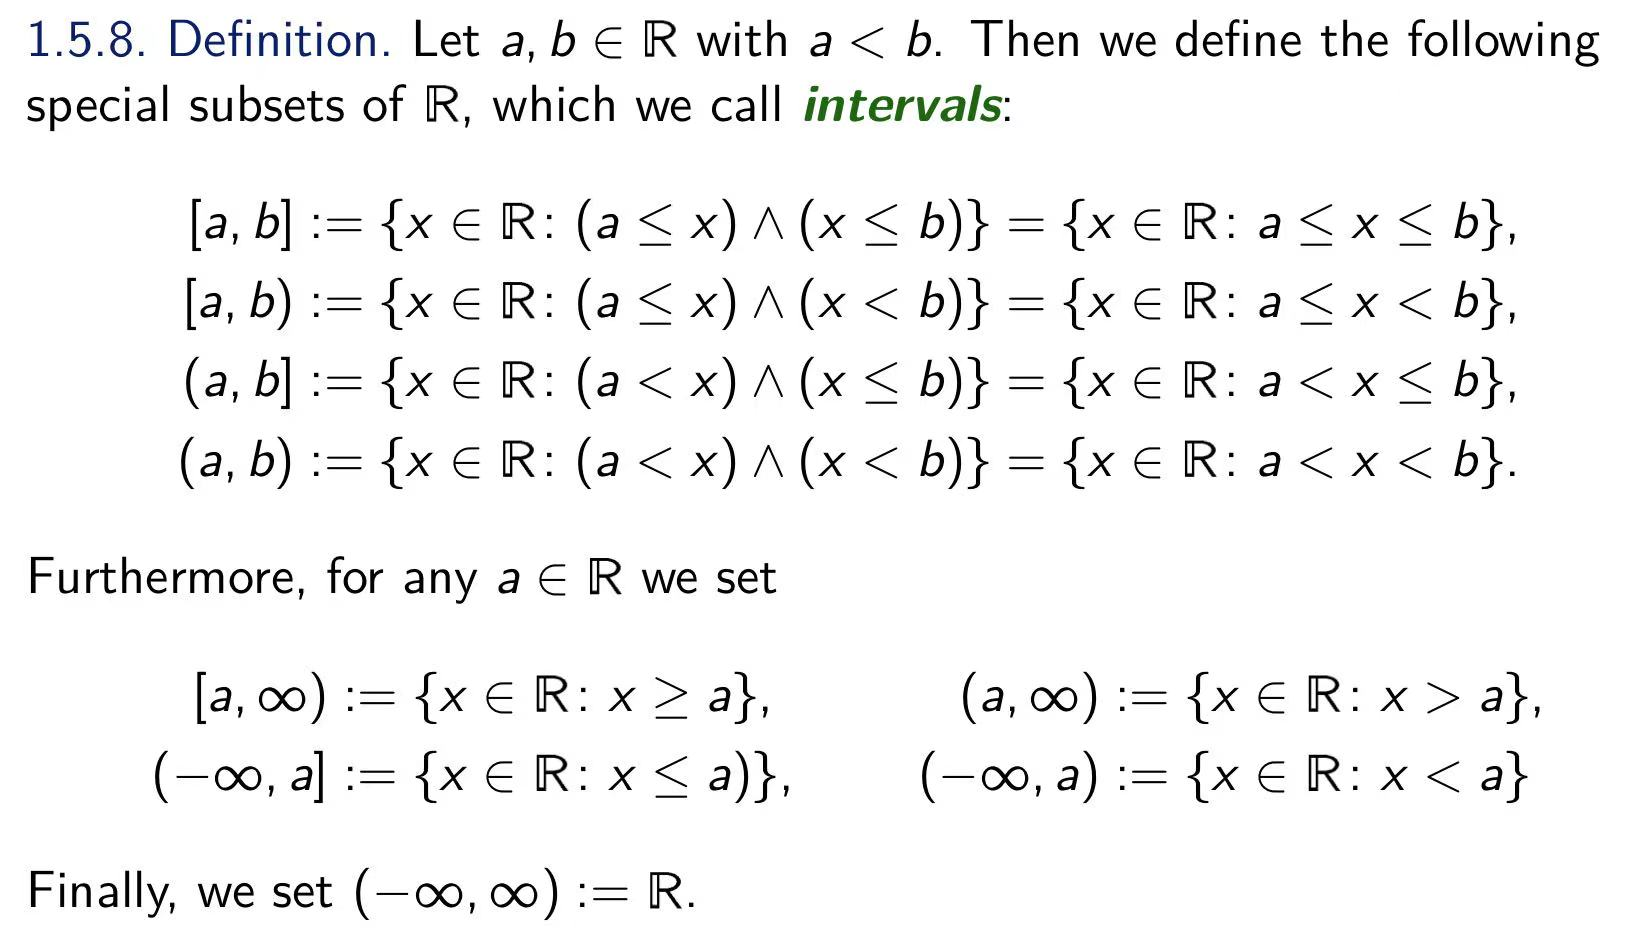
\includegraphics[width=12cm]{interval.jpg}
    \end{figure}

\end{frame}
\begin{frame}
    \frametitle{Sets \& Points}
    Recall the following definition and notation, it is very likely to appear in your exam !
    \begin{itemize}
        \item Interior point
        \item Exterior point
        \item Boundary point
        \item Accumalation point
    \end{itemize}

    For each kind of points, discuss whether the point should be in the set or not ?

    Whether a boundary point for a set must be an accumalation point for a set ?

    \vspace{0.5em}
    Tips:\\
    \begin{itemize}
        \item \textbf{Remember the definitions!}\\
        \item \textbf{Draw the pictures!}\\
        \item \textbf{Pay attention to some speacial cases!}
    \end{itemize}
\end{frame}

\begin{frame}
    \frametitle{Better understand accumulation point}
    \begin{itemize}
        \item Try to prove that : if x is an accumulation point of set A, for every $\epsilon \textgreater 0$, the set $(x-\epsilon, x+\epsilon)\cap A \backslash \{x\}$ contains infinite elements.
        \item Consequently, you can take elements from the set to construct a sequence that converges to x.
    \end{itemize}
\end{frame}

\begin{frame}
    \frametitle{Examples in class}
    Those two examples can give us some thought.
    \begin{figure}[htbp]
        \centering
        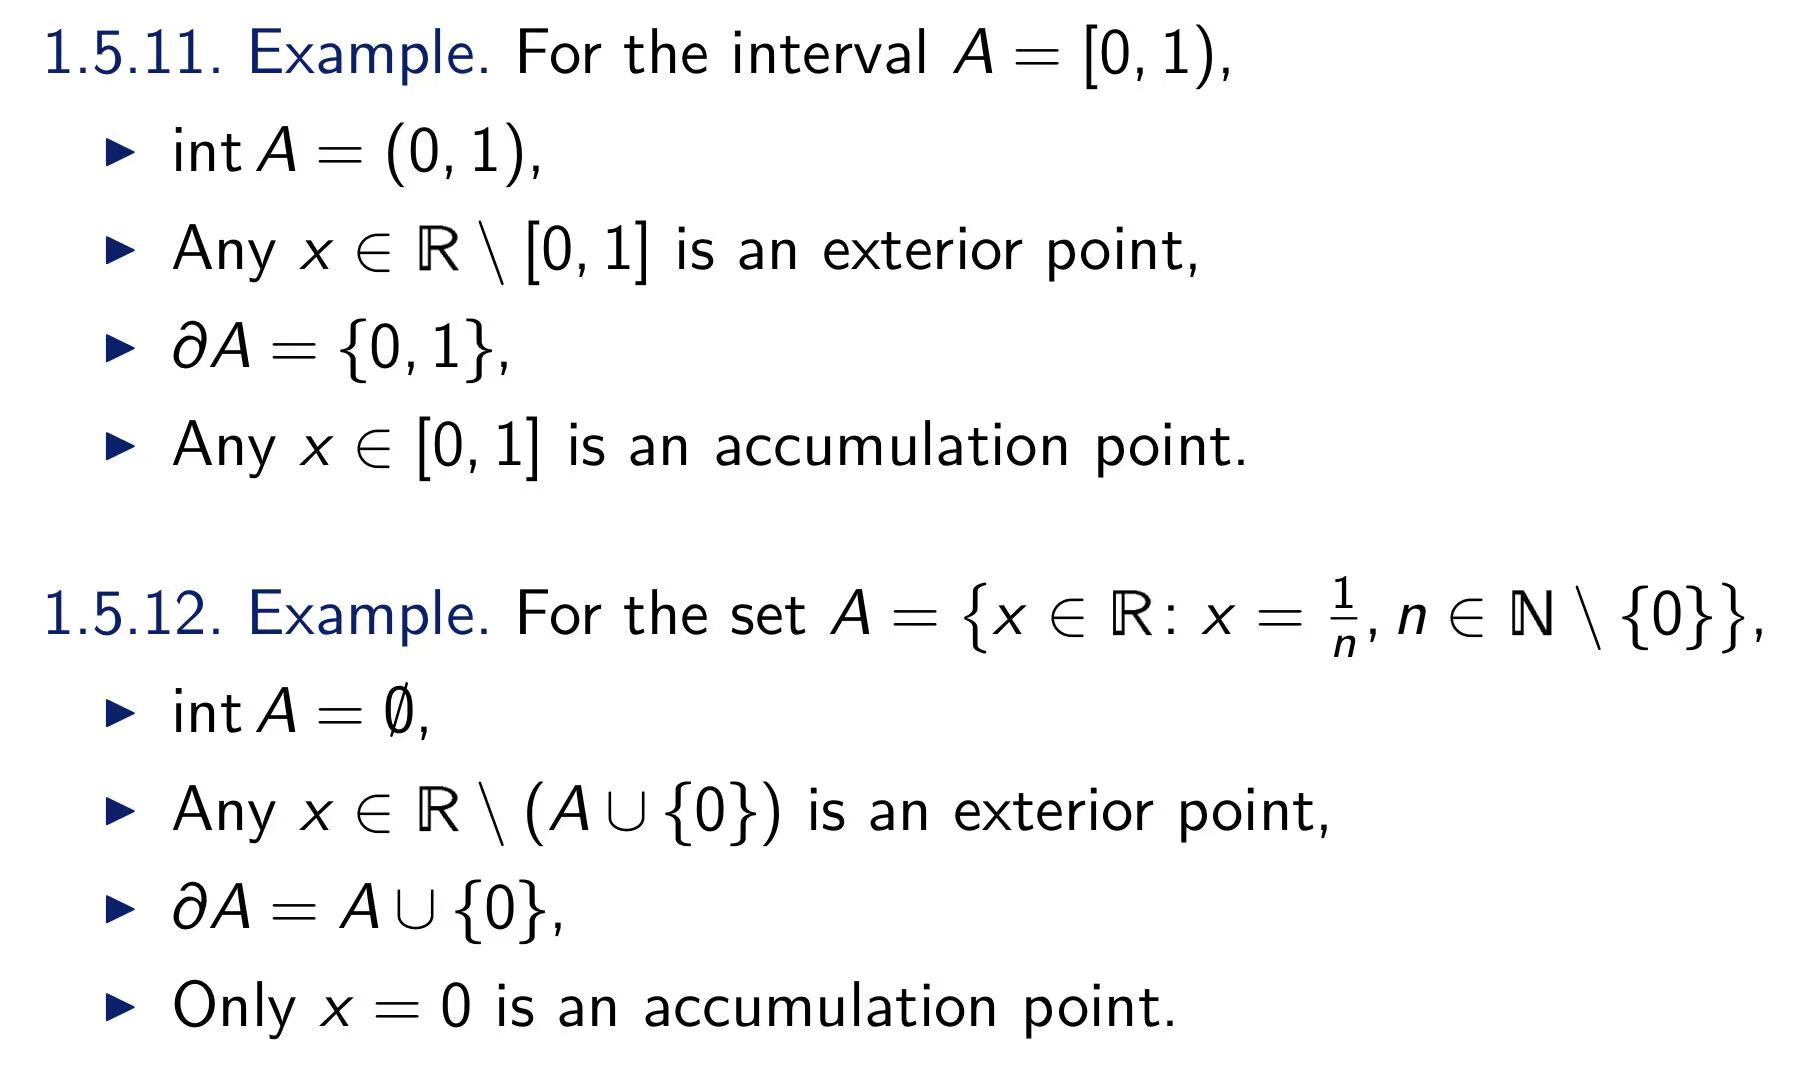
\includegraphics[width=10cm]{example.jpg}
    \end{figure}
\end{frame}

\begin{frame}
    \frametitle{Exercise about points}
    Please identify the interior, exterior, boundary and accumalation
    points of the set
    $$\{\frac{1}{z}:z\in \mathbb{Z}\backslash\{0\}\}\cup (\bigcap_{j=1}^\infty(-2-\frac{1}{j},-1+\frac{1}{j}))$$
\end{frame}

\begin{frame}
    \frametitle{Sets \& Points}
    Recall the following definition:
    \begin{itemize}
        \item Open Set
        \item Closed set
        \item Closure
    \end{itemize}
    Remark: Remember that a set does \textbf{NOT} have to be either open or closed.
\end{frame}

\begin{frame}
    \frametitle{Conceptual Exercises}
    Please judge true or false:
    \begin{itemize}
        \item The set $\mathbb{R}$ is an open set ?
        \item The set $\mathbb{R}$ is a closed set ?
        \item An empty set is an open set ?
        \item An empty set is a closed set ?
        \item The set $(a,b]$ is an open set or a closed set ?
        \item The set $\{x\in \mathbb{R}: x=\frac{1}{n}, n\in \mathbb{N}\backslash\{0\}\}$ is closed ?
    \end{itemize}
\end{frame}

\begin{frame}
    \frametitle{Boundness}
    How we define those concepts for a set ?
    \begin{itemize}
        \item bounded/unbounded
        \item max/min
        \item sup/inf
    \end{itemize}
    \begin{block}{Quick check:}
        \begin{itemize}
            \item 1. What's the relationship between max/min and sup/inf.
            \item 2. Does max/min or sup/inf always exists for bounded sets? When ?
        \end{itemize}
        Important Conclusion: inf S = $\xi \in S \Leftrightarrow \xi=$ min S
    \end{block}
    \vspace{1em}
    \textbf{Get familiar with this!}
\end{frame}



\begin{frame}
    \frametitle{Boundness}
    Check the scope ! Q or R ......

    \textbf{Example:}\\
    \begin{enumerate}
        \item The set $A=(-\infty, a)$ is bounded above in $\mathbb{R}$ with $\sup A=a$. It isn't in $A$.
        \item The set $B=[b,+\infty)$ is bounded below in $\mathbb{R}$ with $\inf B=b$. It's in $B$ since $b$ is the minimum of $B$.
        \item The set $C=[c,d)\cup(e,f)$ is bounded above and below in $\mathbb{R}$, so it's bounded with $\sup C=f$, $\inf C=c$.
        \item The set $D=\{x\in \mathbb{Q}^+: x=\frac{1}{n}, n\in \mathbb{N}^*\}$ is bounded above in $\mathbb{Q}^+$, but not bounded
              below in $\mathbb{Q}^+$.
    \end{enumerate}
\end{frame}

\begin{frame}
    \frametitle{Exercise}
    The conclusion is really useful, we will frequently use it !
    \begin{figure}[htbp]
        \centering
        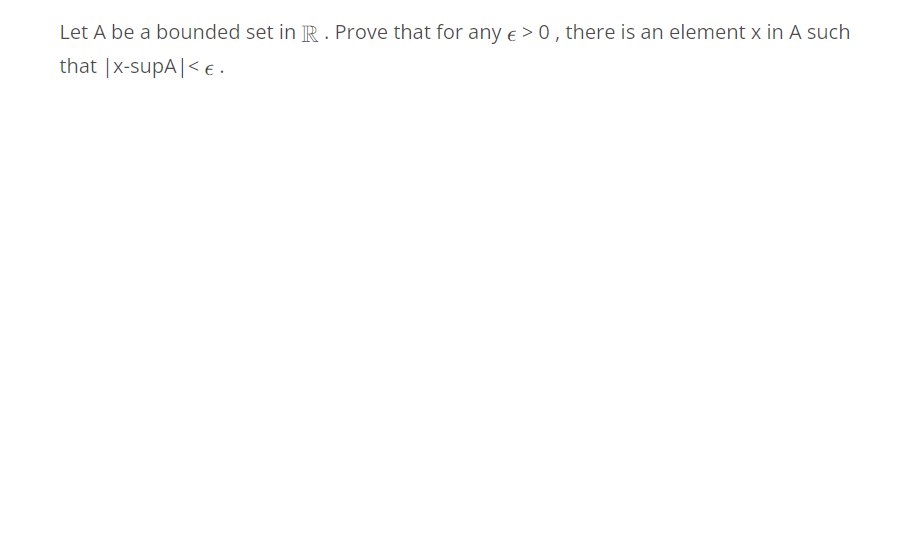
\includegraphics[width=12cm]{exercise2.png}
    \end{figure}
\end{frame}


\begin{frame}
    \frametitle{Tips on proving a supremum or infimum}
    Generally, proving $\eta$ is a supremum of a set S has two steps:
    \begin{enumerate}
        \item Firstly, show that $\eta$ is a upper bound for S. i.e. $\forall x \in S, x\leq \eta$.
        \item Secondly, show that $\forall \alpha \textless \eta, \exists x_{0} \in S, x_{0} \textgreater \eta$.
    \end{enumerate}

    Sometimes an inequality is useful (directly come from the definition):
    \begin{itemize}
        \item For a set S, if $\forall x \in S, x \leq y,$ then sup S $\leq$ y.
    \end{itemize}
    The steps for proof and properties for infimum is quite similar to supremum.
\end{frame}

\begin{frame}
    \frametitle{Exercise}
    \begin{figure}[htbp]
        \centering
        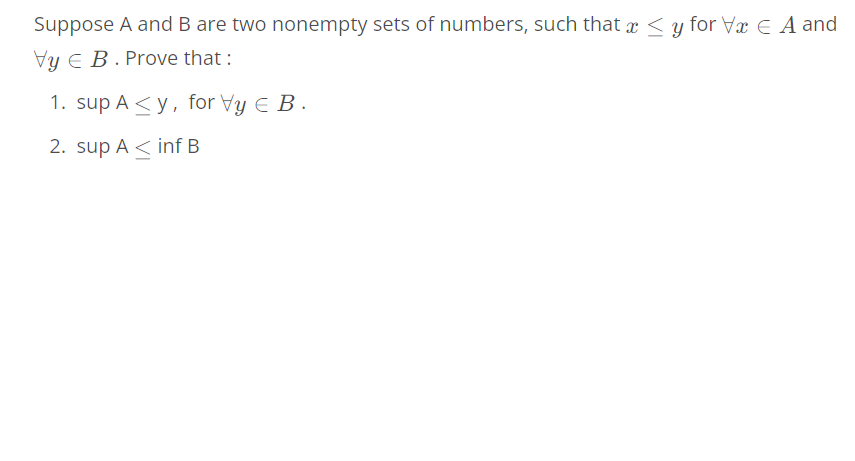
\includegraphics[width=12cm]{exercise4.png}
    \end{figure}
\end{frame}

\begin{frame}
    \frametitle{Exercise}
    \begin{figure}[htbp]
        \centering
        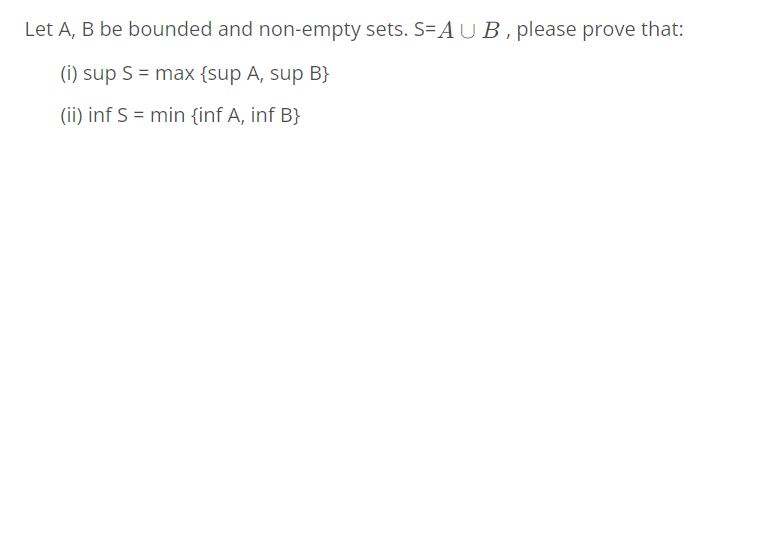
\includegraphics[width=12cm]{exercise3.png}
    \end{figure}
\end{frame}

\begin{frame}
    \frametitle{Exercise}
    \begin{figure}[htbp]
        \centering
        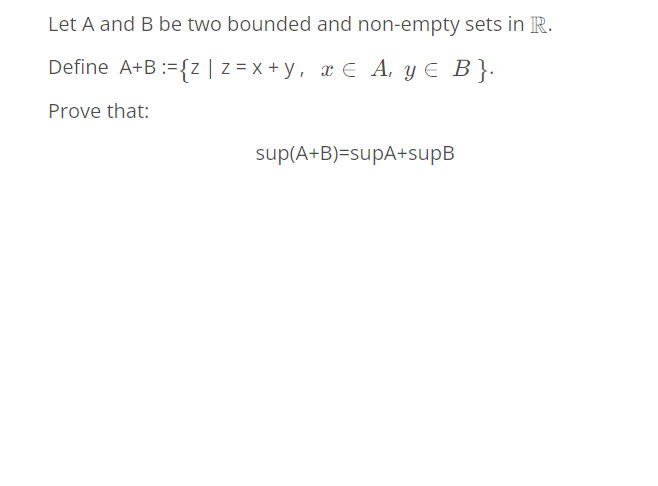
\includegraphics[width=12cm]{exercise.png}
    \end{figure}
\end{frame}

\section{Rational Nums}
\begin{frame}
    \frametitle{Rational Numbers}
    \hspace{1em}
    We define that the set of rational numbers is
    \begin{equation*}
        \mathbb{Q}=\{\frac{p}{q}:p,q\in \mathbb{Z}\wedge q \neq 0\}
    \end{equation*}
    together with the following properties(P1-P9).
    \begin{table}
        \centering
        \resizebox{10cm}{!}{%
            \begin{tabular}{cccc}
                \toprule
                $Porperties$      & \multicolumn{1}{c}{Addition}                         &  & \multicolumn{1}{c}{Multiplication}    \\
                \midrule
                $Associativity$   & $a+(b+c)=(a+b)+c$                                    &  & $a\cdot (b\cdot c)=(a\cdot b)\cdot c$ \\
                \\
                $Neutral Element$ & $a+0=0+a=a$                                          &  & $a\cdot 1=1\cdot a=a$                 \\
                \\
                $Commutativity$   & $a+b=b+a$                                            &  & $a\cdot b=b\cdot a $                  \\
                \\
                $Inverse Element$ & $(-a)+a=a+(-a)=0$                                    &  & $a\cdot a^{-1}=a^{-1}\cdot a=1$       \\
                \\
                $Distributivity$  & \multicolumn{3}{c}{$a\cdot (b+c)=a\cdot b+a\cdot c$}                                            \\
                \bottomrule
            \end{tabular}%
        }
    \end{table}
\end{frame}

\begin{frame}
    \frametitle{Rational Numbers}
    Property 10: Trichotomony Law (Using a set P to divide Q into three parts)

    Property 11 and 12: Feature the set P, such that positive numbers are closed under addition and multiplication
\end{frame}

\begin{frame}
    \frametitle{Important Inequality}
    For all rational numbers $a,b\in \mathbb{Q}$, we have
    $\left|\left|a\right|-\left|b\right|\right|\leq \left|a+b\right|\leq \left|a\right|+\left|b\right|$

    \vspace{2em}
    Prove it using Mathematical Induction !

    Corollary: $\left|\sum_{i=1}^n a_{i}\right|$ $\leq$ $\sum_{i=1}^n \left|a_{i}\right|$
\end{frame}

\begin{frame}
    \frametitle{The Square Root Problem}
    \hspace{1em}
    Let $M=\{t \in \mathbb{R} : t>0 \wedge t^2>x \}, y=\inf M.$
    We want to prove that $y^2=x$ by showing that $y^2 > x$ and $y^2<x$
    lead to contradictions.
    \begin{figure}[htbp]
        \centering
        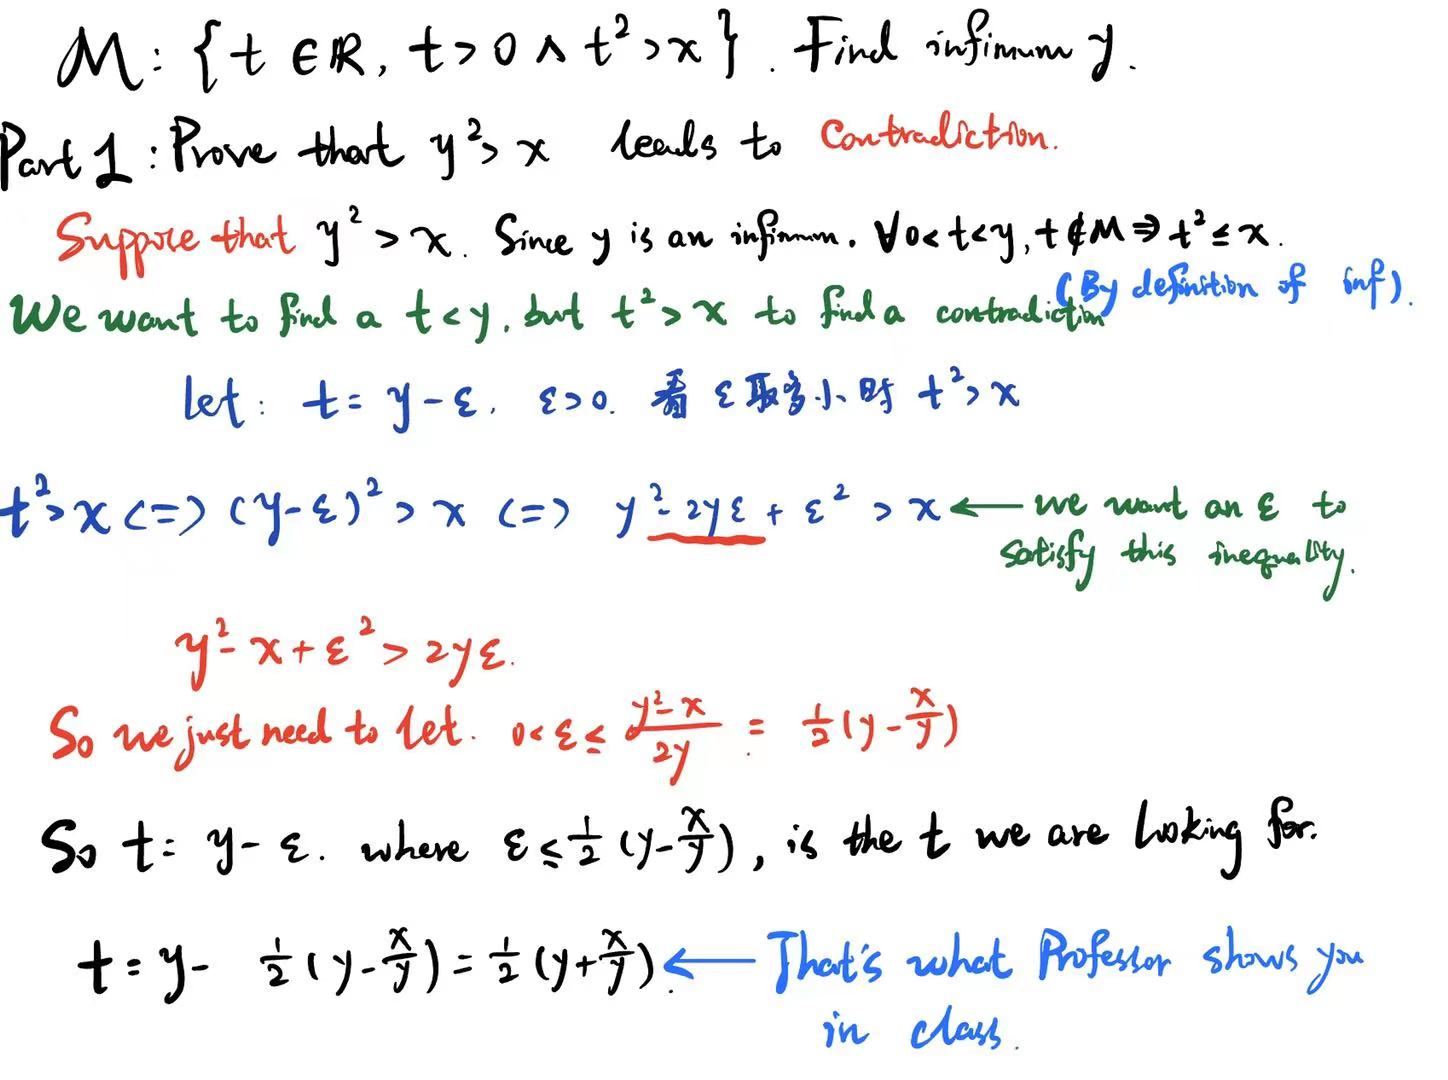
\includegraphics[width=12cm]{squareProblem.jpg}
    \end{figure}
\end{frame}

\begin{frame}
    \frametitle{Part 2 for contradiction}
\end{frame}

\begin{frame}
    \frametitle{Important Conclusion}
    Infimum and Supremum don't necessarily exist in a bounded set defined in Q.
\end{frame}

\section{Real Numbers}
\begin{frame}
    \frametitle{Real Numbers and Important Conclusion}
    The square root problem tells us that: Bounded sets may not have infimum or supremum.

    The definition of real numbers guarantees that for a set in $\mathbb{R}$, \textbf{if it is bounded above, then it has an supremum;
        if it is bounded below, then it has a infimum.}

    \begin{figure}[htbp]
        \centering
        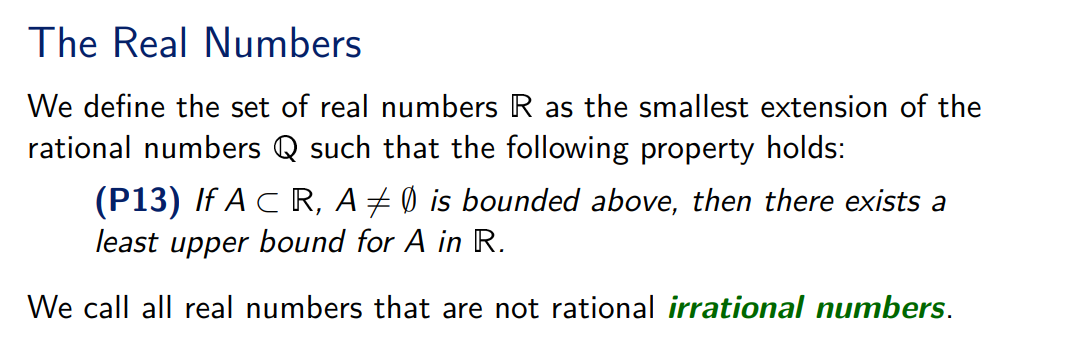
\includegraphics[width=12cm]{definition.png}
    \end{figure}
\end{frame}


\begin{frame}
    \frametitle{Complex Numbers}
    \hspace{1em}
    In Vv186, you just need to know how to perform basic complex numbers' computation
    and some basic properties.
    Here, we just list some basic computation rules and formulas.\\
    Given $z_1=(a_1,b_1)$ and $z_2=(a_2,b_2)$,
    \begin{itemize}
        \item $z_1+z_2=(a_1,b_1)+(a_2,b_2)=(a_1+a_2,b_1,b_2)$
        \item $z_1\cdot z_2=(a_1,b_1)\cdot (a_2,b_2)=(a_1a_2-b_1b_2,a_1b_2-a_2b_1)$
        \item $c\cdot z_1=c(a_1,b_2)=(ca_1,cb_1), c\in \mathbb{R} $
        \item $\bar{z_1}=(a_1,-b_1)$
        \item $|z_1|^2=a_1^2+b_1^2=z_1\bar{z_1}$
        \item Re $z_1= \frac{z_1+\bar{z_1}}{2}$
        \item $($Im $z_1 )i= \frac{z_1-\bar{z_1}}{2}$
    \end{itemize}
\end{frame}

\begin{frame}
    \frametitle{Open Ball}
    Let $z_0 \in \mathbb{C}$. Then we define the \textbf{\textcolor{blue}{open} \textcolor{red}{ball}} of radius
    $R>0$ centered at $z_0$ by
    $$B_R(z_0):=\{z \in \mathbb{C} :|z-z_0|<R\}$$

    \begin{itemize}
        \item Geometric interpretation?
        \item Higher dimensions?
    \end{itemize}

    How to define the boundness of a set in $\mathbb{C}$ ?

    Are there lower bound or upper bound for a bounded set in $\mathbb{C}$ ?

\end{frame}

\section{Function}
\begin{frame}
    \frametitle{Important Definition for Function}
    Recall the definition of domain, codomain and range.

    \vspace{1em}
    Let's start from the notation for functions.

    \vspace{1em}
    \begin{center}
        $f:\varOmega \rightarrow Y$, \qquad $x\mapsto f(x)$.

        \vspace{1em}
        or alternatively

        \vspace{1em}
        $f:\varOmega \rightarrow Y$, \qquad y = f(x).
    \end{center}

    Example: Point out the domain, codomain and range for the function:

    \begin{center}
        $f:\mathbb{R}^2 \rightarrow \mathbb{R}$, \qquad  f(x,y)=$x^{2}+y^{2}$
    \end{center}
\end{frame}


\section{Extra Exercise}

\begin{frame}
    \frametitle{Exercise}

    We will spend some time discussing about $\overline{lim}$ and $\underline{lim}$, and their relation with sup/inf for sets in next RC.
    \begin{figure}[htbp]
        \centering
        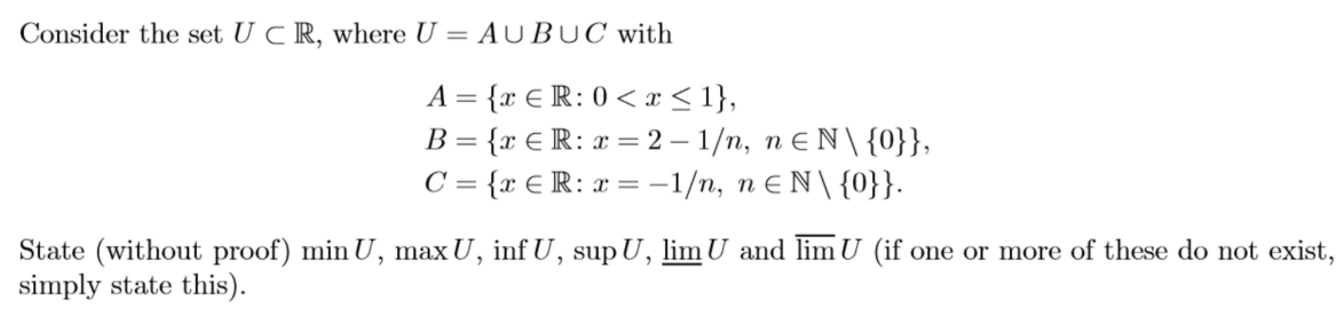
\includegraphics[width=12cm]{extra2.png}
    \end{figure}
\end{frame}

\begin{frame}
    \frametitle{Exercise}
    \begin{figure}[htbp]
        \centering
        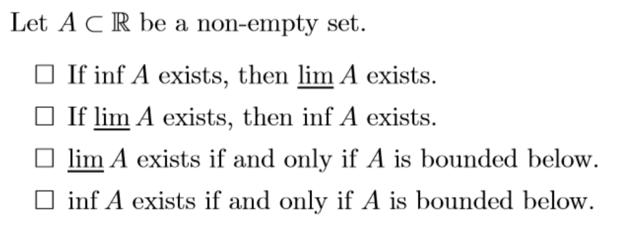
\includegraphics[width=12cm]{extra.png}
    \end{figure}
\end{frame}

\section{Reference}
\begin{frame}
    \frametitle{Reference}
    \begin{itemize}
        \item Exercises from 2021-Vv186 TA-Ni Yinchen.
        \item Exercises from 2021-Vv186 TA-Tu Yiwen.
        \item Exercises from 2022-Vv186 TA-Sun Meng
    \end{itemize}
\end{frame}
\end{document}